\pagebreak
\section{Use Cases in Internet of Things}

Deploying virtual-kubelet to an IoT device is a double-edged sword. On the one hand, it easily migrates development effort of Kubernetes' communication to IoT. You get security and interoperability out of the box. For every possible state of your end-device, there is a predefined Kubernetes description that matches with it. That allows solutions for cloud environments to co-operate with end-devices, such as the \textit{NodeWatcher} program explained before. On the other hand, Kubernetes ecosystem is not build for resource-constraint devices. The communication protocol between kubelets and Kubernetes master is HTTPS. While it's secure, it's more resource hungry than other popular IoT messaging systems such as MQTT. As discussed above, projects like FLEDGE overcome this problem by deploying virtual-kubelet to the cloud and using MQTT to connect to devices. An e-mail exchange with one of the FLEDGE authors revealed that they are migrating their codebase to deploy virtual-kubelet on the end device. It's up to the developers to decide which one is more suitable for their system. If they are using large clusters with weak end-devices such as microcontrollers, it's better to deploy virtual-kubelet to the cloud and deploy a more lightweight agent to end-device. If they have relatively powerful devices, such as Raspberry Pi, it makes more sense to deploy virtual-kubelet to the them.

Additional to the Raspberry Pi example in the \hyperref[chapter:implementation]{implementation} section, another example was developed to show the interaction between unikernels and sensors. A python script was created to read sensor data from multiple sensors and write it to respective files. Unikernels can be programmed to read sensor data directly from GPIO pins, but implementation of a driver for MirageOS is out of scope for this project. Unikernels in the example read sensor data from files instead. The name of the respective sensor file is given in the deployment specification of the unikernel and then it's passed as an environment variable to the running application. Full code for the application can be seen in \ref{fig:ocaml-demo}. This code is accompanied with a config file which determines names of input arguments and lists dependencies. It becomes obsolete once the application is compiled and the binary can be distributed standalone. It takes 2.6 MB when compiled for unix. Complete deployment specification for a unikernel that reads humidity sensor can be found in \ref{fig:unikernel-dep}.

For IoT scenarios involving devices where virtualisation is possible, unikernels tell a much different story. They have a smaller size when compiled for hypervisors (seen in \ref{tab:sizes}), thus have a faster distribution rate among devices. They can communicate with other unikernels on the same device by sharing volumes, which is a trivial task for modern hypervisors. They are also booted faster on hypervisors. Combined with their smaller size, this means less delay when updating software on those devices. 

\begin{figure}[htpb]
    \centering
    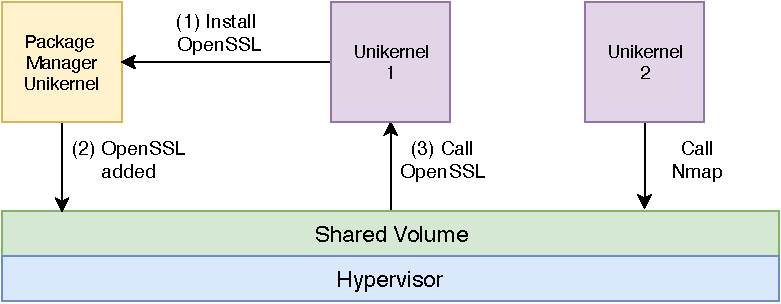
\includegraphics[width=0.9\textwidth]{packagemanager.pdf}
\caption{A package manager for external dependencies}\label{fig:package}
\end{figure}


A shortcoming of unikernels when compared with Docker containers running on end-devices is their inability to encapsulate dependencies. If a Docker application needs OpenSSL, it comes bundled with its image but in current unikernel technology that is not possible. A workaround is to deploy dependencies on devices beforehand and make unikernels call those programs externally. This is possible on hypervisors by mounting the executables folder to the unikernel instance. Nevertheless, it requires dependencies to be static during development so that they can be installed on the device. If that is not possible, a dedicated unikernel with write access to executables folder can work as a package manager by installing dependencies of every running instance from the internet. The solution can be seen in figure \ref{fig:package}.

The external dependencies of a unikernel application can be stated as labels in the deployment specification. Virtual-kubelet can be modified to send those dependencies directly to package manager unikernel or it can act directly as the package manager. Despite that solution, calling a program through a shared volume is a slow process. Unikernel developers have to come up with a solution to directly embed libraries inside their images.